\documentclass{article}
\usepackage[utf8]{inputenc}

\usepackage{amsthm,amssymb,amsmath,mathtools}
\usepackage{graphicx}
\usepackage{subfigure}
\usepackage{hyperref}


\newtheorem*{theorem}{Theorem}

%% custom command definitions 
% transpose
\def \T {{\mathsf{T}}}

% variables
\def \s {{\mathbf{s}}}

% domain
\def \R {{\mathbb{R}}}


\title{UWB Sensor Coverage Analysis}
\author{Lavish Arora} % Replace Me with your name!
\date{\today}

\begin{document}

\maketitle

%%%%%%%%%%%%%%%%%%%%%%%%%%%%%%%%%%%%%%%%%%%%%%%%%%%%%%%%%%%%%%%%%%%%%%%%%%%%%%
This report discusses the placement of UWB sensors for maximizing the tracking coverage in an area. We start by discussing a simplistic 2D case and the ideas is to extend the approach to a more realistic 3D case.

\section{The Sensor model}

The UWB sensor is an RF chip whose antenna has certain directional wave propagation characteristics leading to a typical coverage for the sensor. We consider a conservative yet simplistic model of a UWB anchor node shown in fig. \ref{fig:uwb-pro}, we could have also chosen a double sided parabolic profile instead of a double sided triangular this provides a conservative estimate rather than overestimating the coverage.

\begin{figure}[!h]
	\centering
	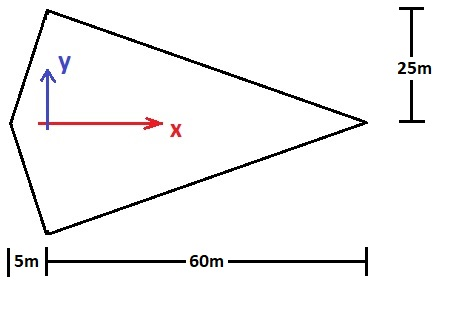
\includegraphics[scale=0.6]{img/uwb-sensor-profile.jpg}
	\caption{A simplistic and yet conservative coverage model of a single UWB sensor, the sensors x and y axis are shown in red and blue respectively}
	\label{fig:uwb-pro}
\end{figure}

%%%%%%%%%%%%%%%%%%%%%%%%%%%%%%%%%%%%%%%%%%%%%%%%%%%%%%%%%%%%%%%%%%%%%%%%%%%%%%
\section{Core assumptions}

We assume that whenever the target node is in the tracking area of the anchor node a ranging measurement can be generated. For a target node to be localized we will consider that at least range measurements from four anchors are required. An area is covered if each point in the area is in FOV of at least 4 anchors.


%%%%%%%%%%%%%%%%%%%%%%%%%%%%%%%%%%%%%%%%%%%%%%%%%%%%%%%%%%%%%%%%%%%%%%%%%%%%%%
\section{Related work}

This problem is related to the classical polygon covering problem [1] with different objective which becomes a special case of set cover problem. We also here have constraints that the individual primitive units used to cover the polygon do not overlap exactly, as overlapping sensors do not help in localization and measurements should arrive from sensors placed at different locations.

Further literature review is required to look at the current methods to solve the problem. There are few works [2-4] that look at the problem at hand and mainly focus on minimizing the lower bound on the localization uncertainty of the targets. A detailed study of them is required.

%%%%%%%%%%%%%%%%%%%%%%%%%%%%%%%%%%%%%%%%%%%%%%%%%%%%%%%%%%%%%%%%%%%%%%%%%%%%%%
\section{Preliminary Formulation}

Let there be $n$ sensors in 2D space with $i^{th}$ sensor placed at $\s_i \in \text{SE(2)}$ for all $1\leq i\leq n$. A point $p$ with coordinates $(x_p,y_p) \in \R^2 $ in space is said to be covered by the $i^{th}$ sensor if the point falls in the sensors range. 

Before stating the problem at hand we define a few functions.

\paragraph{Indicator function}
We define the indicator function $c_p(\s_i)$ as follows
\begin{equation}
	c_p(\s_i) \coloneqq 
	\begin{cases}
		1 & \text{if point $p$ in $i^{th}$ sensor range}\\
		0 & \text{otherwise}
	\end{cases}
\end{equation}


\paragraph{Special Polynomials}
Special polynomials $f_k(x_1,x_2,\dots,x_n)$ in $n$ variables $x_1,x_2,\dots,x_n$ for $k=1,\dots,n$ are defined as

\begin{equation}
	\begin{aligned}
		& f_1(x_1,x_2,\dots,x_n) \coloneqq 1-\prod_{1\leq i\leq n} (1 - x_i) \\
		& f_2(x_1,x_2,\dots,x_n) \coloneqq 1-\prod_{1\leq i < j \leq n} (1 - x_ix_j) \\
		& . \\
		& f_4(x_1,x_2,\dots,x_n) \coloneqq 1-\prod_{1\leq i < j < k < l <\leq n} (1 - x_i x_j x_k x_l) \\
		& \vdots \\
		& f_n(x_1,x_2,\dots,x_n) \coloneqq x_1 x_2 \dots x_n
	\end{aligned}
\end{equation}
for general $k$ we define $f_k(x_1,x_2,\dots,x_n)$ as
\begin{equation}
	f_k(x_1,x_2,\dots,x_n) \coloneqq 1 - \prod_{1\leq j_1 < j_2 < \dots < j_k \leq n} (1 - x_{j_1} x_{j_1} \dots x_{j_1})
\end{equation}
for $k=1,\dots,n$. These special polynomials help us formulate the general $k$-coverage problem.

\subsection{$k$-coverage problem}
We sample $m$ points from the area of interest using a uniform distribution. For a point $p^j$ at location $(p^j_x,p^j_y)$ to be $k$-covered it has to be in range of atleast $1\leq k\leq n$ sensors. This can mathematically expressed as an indicator function $f_k(c_{p^j}(\s_1),c_{p^j}(\s_2),\dots,c_{p^j}(\s_n))$ over the position of $n$ sensors $\{\s_i\}_{i=1}^n$. 

We would like to maximize the $k$-coverage of all the sampled points in the space of interest. Which leads to the following maximization problem for finding the optimal sensor placement. Let $S \coloneqq [\s_1^\T \s_2^\T \dots \s_n^\T]^\T$

\begin{equation}\label{kcov}
	S^* = \arg \max_{S} \sum_{j=1}^{m} f_k(c_{p^j}(\s_1),c_{p^j}(\s_2),\dots,c_{p^j}(\s_n))
\end{equation}


%%%%%%%%%%%%%%%%%%%%%%%%%%%%%%%%%%%%%%%%%%%%%%%%%%%%%%%%%%%%%%%%%%%%%%%%%%%%%%
\section{Methodology}

\subsection{Heuristic method}
Initially we look at a simplistic case of solving the problem for two specific settings $80 \times 65 m^2$ and  $120 \times 90 m^2$ rectangular spaces. The following are the goals of the UWB placement problem:
\begin{enumerate}
	\item Maximize tracking area coverage
	\item Use as less number of sensors as possible
\end{enumerate}

One could in practice cover the whole area by using a large number of sensors but the idea is to have the maximum (typically $\geq$ 90\%) coverage while minimizing the number of sensors.
Ideally, we would like to solve an optimization problem but in this text we resort to simple heuristics to solve the problem. We implemented a scheme for sensor placement using the following approach:
\begin{enumerate}
	\item start by placing sensors on the corners of the rectangular space pointing towards the opposite vertex.
	\item place sensors in the middle of the edges pointing towards the center of the space.
	\item check coverage using the MATLAB tool and add sensors generously on the edges in between two sensors pointing towards an area less covered.
	\item place sensors inside the space where the coverage seems to be low.
	\item repeat until the required coverage threshold is achieved
	\item tweak angles of sensors and check in tool if it improves coverage
	\item check for the least important sensor by removing each sensors one by one and see the effect on coverage and repeat until a lower bound on the required coverage is reached.
\end{enumerate}

\subsection{Solving the $k$-coverage problem}
The $k$-coverage problem in \ref{kcov} is non-convex, non-differentiable and may have multiple solutions. We may look at ways to smooth the problem by considering a smooth sensor model and exploit the finite sum structure to solve it efficiently.

%%%%%%%%%%%%%%%%%%%%%%%%%%%%%%%%%%%%%%%%%%%%%%%%%%%%%%%%%%%%%%%%%%%%%%%%%%%%%%%
\section{Results for Heuristic method}

\begin{figure}
	\centering
	\subfigure{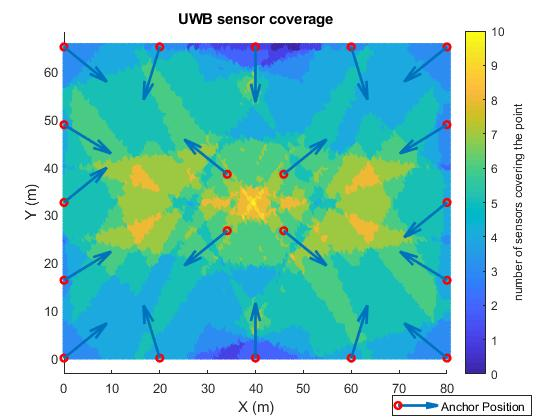
\includegraphics[scale=0.3]{img/uwb-env1.jpg}}
	\subfigure{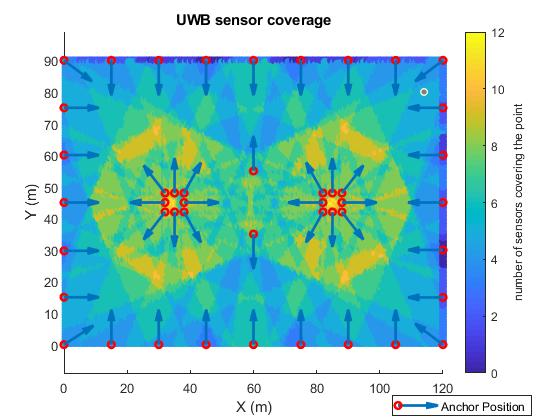
\includegraphics[scale=0.3]{img/uwb-env2.jpg}}
	\caption{Sensor coverage for the $80 \times 65 m^2$ and $120 \times 90 m^2$ environment using the above scheme. The color bar depicting the number of sensors that can reach a given points.}
	\label{fig:uwb-c}
\end{figure}

Here are the results for the two cases following the above procedure. For the first $80 \times 65 m^2$ environment we used 20 sensors and achieved a coverage of 92.3\% while for the $120 \times 90 m^2$ environment which is approximately double in area we ended up using 46 sensors and were able to achieve a coverage of more than 97.5\%. 

\begin{figure}[!h]
	\centering
	\subfigure{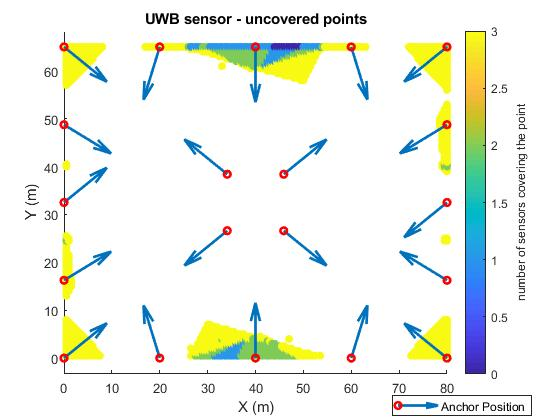
\includegraphics[scale=0.3]{img/uwb-coverage-env1.jpg}}
	\subfigure{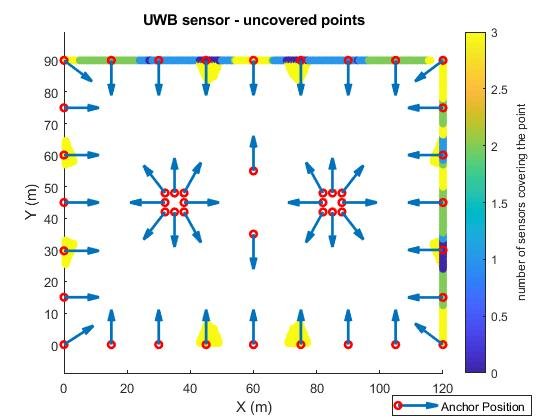
\includegraphics[scale=0.3]{img/uwb-coverage-env2.jpg}}
	\caption{Figure displaying uncovered points for the $80 \times 65 m^2$ and $120 \times 90 m^2$ environment using the above scheme. The white portion is the covered region and the colored region depict the uncovered region with the color bar depicting the number of sensors that can reach the uncovered points.}
	\label{fig:uwb-u}
\end{figure}

\noindent The MATLAB code used here can be accessed here: \href{https://github.com/Muskman/uwb-tools}{https://github.com/Muskman/uwb-tools}

\section*{References}

[1] “Polygon Covering.” Wikipedia,  1 May 2020, \textit{en.wikipedia.org/wiki/Polygon\_covering}. \\

\noindent[2] Sadeghi, Mohammad, Fereidoon Behnia, and Rouhollah Amiri. "Optimal Sensor Placement for 2-D Range-only Target Localization in Constrained Sensor Geometry." \textit{IEEE Transactions on Signal Processing (2020)}. \\

\noindent[3] Yang, Chun, et al. "Optimal placement of heterogeneous sensors for targets with Gaussian priors." \textit{IEEE Transactions on Aerospace and Electronic Systems (2013)}. \\

\noindent[4] Jourdan, Damien B., and Nicholas Roy. "Optimal sensor placement for agent localization." \textit{ACM Transactions on Sensor Networks (2008)}.

\end{document}
